\begin{center}
\begin{tikzpicture}

    \begin{scope}[x={(current page.south east)},y={(current page.north west)}]
    	\node[anchor=south,inner sep=0] (image)  at (0.5,0.0) {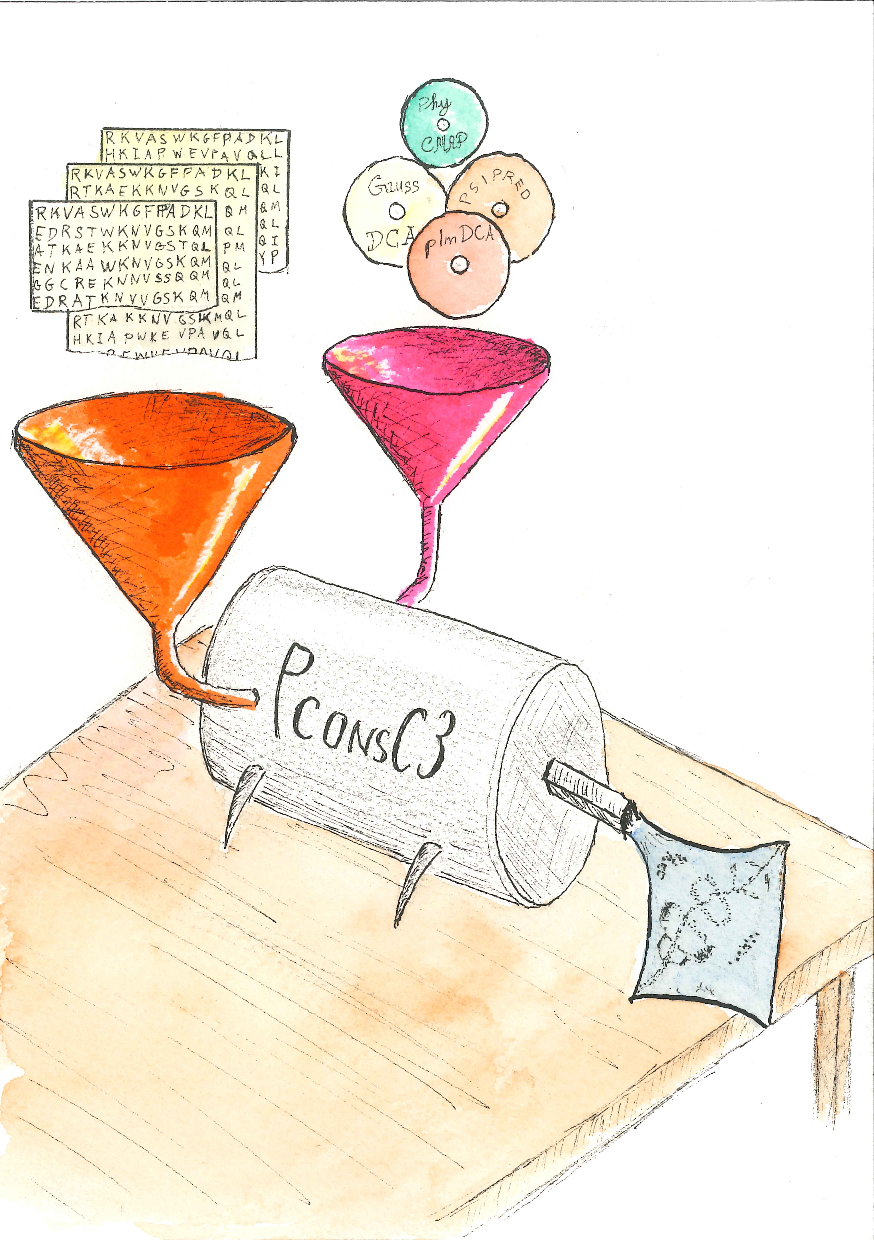
\includegraphics[trim={2mm, 22mm, 2mm, 2mm}, clip, width=0.98\pagewidth]{scans/panel-4.pdf}};
		\if\helplines1
			\draw[help lines,xstep=.1,ystep=.1] (0,0) grid (\N, \N);
		\else
			\path[help lines,xstep=.1,ystep=.1] (0,0) grid (\N, \N);
		\fi
		\node(title) at (0.5, 0.9) {\Huge {\color{Maroon}III} - PconsC4};
		
		
		\node[text width=0.3\pagewidth, align=justify, anchor=north west] at (0.65, 0.8) {\english{The previous paper predicted contacts using a program called PconsC3.
		It combines several multiple sequence alignments, and several independent programs to make its prediction, which makes it slow and difficult to use.}};
		
		\node[text width=0.4\pagewidth, align=justify, anchor=north west] at (0.55, 0.54) {\spanish{El artículo anterior predecía contactos usando un programa llamado PconsC3.
		Combina varios alineamientos múltiples de secuencias, y varios programas independientes, lo que lo hace lento y dificil de usar}};
    \end{scope}

\end{tikzpicture}
\end{center}
